\documentclass{article}

\usepackage{amsmath}
\usepackage{amssymb}
\usepackage{graphicx}
\usepackage{subfigure}
\usepackage{enumerate}
\usepackage{tikz}
\usepackage{qtree}
\usepackage{clrscode3e}
\usepackage{hyperref}
\usepackage{bigstrut}

\pagestyle{plain}

\usepackage[left=3cm,top=2cm,right=3cm,nohead,nofoot]{geometry}

\begin{document}

\begin{center}
\bfseries 685.621 Algorithms for Data Science \\
Homework 3\\
Assigned at the start of Module 6 \\
Due at the end of Module 8 \\
Total Points $100/100$
\end{center}


You are required to participate in the collaborative problem and subproblem separately. Please do not directly post a complete solution, the goal is for the group to develop a solution after everyone has participated. Please ensure you have a write-up with solutions to each problem and subproblems, you are also required to submit code that will be compiled when grading the assignment. In each of the problems you are allowed to use built-in functions.\\

\begin{enumerate}

 %%%%%%%%%%%%%%%%%%%%%%%%% Problem 1 %%%%%%%%%%%%%%%%%%%%%%%%%%%%%%%%%%%%%%%
    \item \textbf{Problem 1 - Module 4 and 5}  \textbf{\emph{This is a Collaborative Problem}}\\
    10 Points Total 

	In this problem use the developed numerical features from HW2. In this problem the following is to be completed:\\

		\item Use the Fisher's Linear Discriminant Ratio (FDR) from the Data Processing document, specifically Equation 20. 
		\begin{enumerate}
			\item (5 points) For each combination of number apply the FDR, e.g., 0 vs 1, 0 vs 2, ..., 0 vs 9, ..., 8 vs 6, 8 vs 7, and 8 vs 9.
			\item (5 points) Place the results in a table. 
		\end{enumerate}

    \vspace{5mm}

	\pagebreak

    %%%%%%%%%%%%%%%%%%%%%%%%% Problem 2 %%%%%%%%%%%%%%%%%%%%%%%%%%%%%%%%%%%%%%%
    \item \textbf{Problem 2 - Module 6}  \textbf{\emph{This is a Collaborative Problem}}\\
    35 Points Total 

	In this problem, you will be developing pseudocode and implementing your development in Python or R for the Expectation Maximization method. You are allowed to use either the Iris data set or the developed numerical features from HW2. In this problem the following is to be completed:\\

  	\begin{enumerate}
		\item (20 points) The development and implementation of the Expectation Maximization method should be for a generic number of clusters, features and observations.
		\item Apply your implementation using either the Iris data or the features generated from HW 2.
		\begin{enumerate}
			\item Use the top two ranked features.
			\item (5 points) Create 3 clusters for the Iris data or 4 clusters using the 4 numerical values that have the best separation.
			\item (5 points) Display the 3 species or 4 numerical values using different colors for a good visual representation.
			\item (5 points) Provide an analysis of your results, e.g., what is your observation of the results, how well did the clusters group each class, etc.
		\end{enumerate}
	\end{enumerate}

    \vspace{5mm}

	\pagebreak

        %%%%%%%%%%%%%%%%%%%%%%%%% Problem 3 %%%%%%%%%%%%%%%%%%%%%%%%%%%%%%%%%%%%%%%
    \item \textbf{Problem 3 - Module 7 - Chapter 1 and 2 [8]} \textbf{\emph{Note this is not Collaborative Problem}}\\
    5 Points Total\\
    
    Define in your own words the following terms: 
    \begin{enumerate}
		\item agent
		\item agent function
		\item agent program
		\item artificial intelligence
		\item autonomy
		\item goal-based agent
		\item intelligence
		\item learning agent
		\item logical reasoning
		\item model-based agent
		\item rationality 
		\item reflex agent
		\item utility-based agent
	\end{enumerate}
    
    \pagebreak


   %%%%%%%%%%%%%%%%%%%%%%%%% Problem 4 %%%%%%%%%%%%%%%%%%%%%%%%%%%%%%%%%%%%%%%
    \item \textbf{Problem 4 - Module 8 - Section 5.3.1 Cross-Validation [7]} \textbf{\emph{This is a Collaborative Problem}}\\
    15 Points Tota\\

	In this problem you are to develop and implement a k-fold cross validation algorithm. You are allowed to use either the Iris data set or the developed numerical features from HW2 to test your implementation. In this problem the following is to be completed:\\
	
	\begin{enumerate}
		\item (5 points) Develop an algorithm to randomly separate data into groups of testing and training groups based on the number of desired folds/experiments, the term used will be k-fold cross validation. Use the 5-fold cross validation in Figure~\ref{fig:fivefold} as a reference. 
		\item (5 points) Implement your k-fold cross validation algorithm.  
		\item (2.5 points) Test your implementation using either the Iris data set or the numerical features generated from HW2.
		\item (52. points) Perform analysis and provide an explanation of how each k-fold creates subsets of the data, e.g., training and testing sets.
	
			\begin{figure}[htbp]
				\begin{center}
    				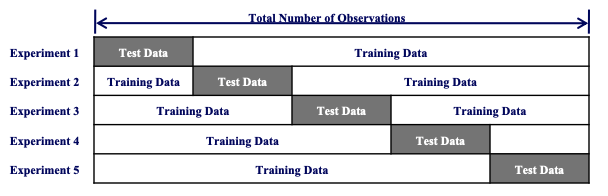
\includegraphics[width=15.2cm]   {fivefold.png}  
    				\caption{5-Fold Cross Validation}
    				\label{fig:fivefold}
				\end{center}
			\end{figure}
	\end{enumerate}

    \vspace{5mm}
    
	\pagebreak

   %%%%%%%%%%%%%%%%%%%%%%%%% Problem 5 %%%%%%%%%%%%%%%%%%%%%%%%%%%%%%%%%%%%%%%
    \item \textbf{Problem 5 - Module 8} \\
    35 Points Total\\
    
The Parzen window algorithm density model is optimized by maximizing the likelihood of the training data with the use of a Gaussian window surrounding each input data point. You are allowed to use either the Iris data set or the developed numerical features from HW2. In this problem the following is to be completed:\\
		\begin{enumerate}
			\item {[15 points]} \textbf{\emph{Note this is not Collaborative Problem}}\\
			Using the Gaussian kernel develop psuedo code to create a Parzen windowing system to accomplish the following steps:
				\begin{enumerate}
					\item Develop and implement the ability to read in data $\textbf{x}_n$ with $n$ observations and $D$ dimensions (number of features).
					\item Using the Gaussian kernel in Eq. 27 of the Machine Learning document to develop and implement an algorithm to process an input observations and compare it with the training observations.
					\item Expand the development and implementation to handle multiple classes.
					\item {[5 point bonus]} use your solution from Problem 4 for a 5-fold cross validation implementation with the Parzen Window. 
				\end{enumerate}
			\item {[5 points]} \textbf{\emph{Note this is not a Collaborative Problem}}
				\begin{enumerate}
					\item Calculate the running time of the system above in $O$-notation.
					\item Calculate the total running time of the above system as $T(n)$ with each line of pseudocode or code accounted for.
					\item How does the total running time $T(n)$ compare to the running time in $O$-notation?
				\end{enumerate}
			\item {[15 points]} \textbf{\emph{Note this is not a Collaborative Problem}}
				\begin{enumerate}
					\item Using all observations and the petal length from the Iris data replicate the subfigures in Figure~\ref{fig:1D_Parzen}.  
					\item Using all observations, the petal length and the petal width from the Iris data replicate the subfigures in Figure~\ref{fig:2D_Parzen}.  
				\end{enumerate}
		\end{enumerate}

\begin{figure}[htbp]
	\begin{center}
    		\subfigure[Gaussian Kernel with h = 0.1] {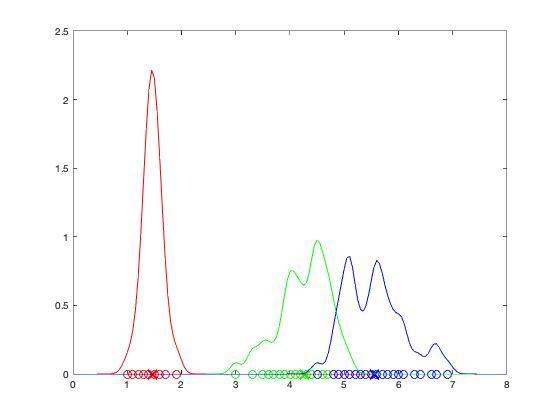
\includegraphics[width=7.6cm]  {gaussianIris0_1.jpg}  \label{fig:gaussianIris0_1}}\\
    		%\hspace{0.1pc}
		\subfigure[Gaussian Kernel with h = 0.25] {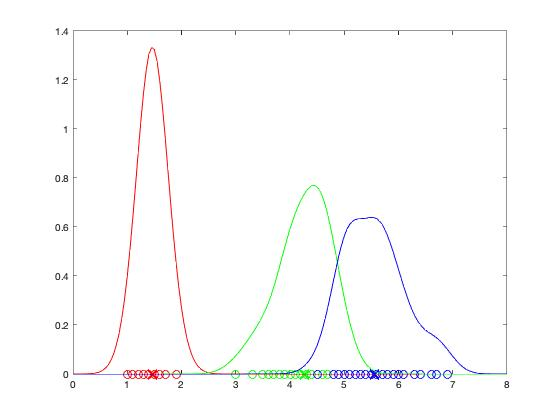
\includegraphics[width=7.6cm]  {gaussianIris0_25.jpg}  \label{fig:gaussianIris0_25}}
    		%\hspace{0.1pc}
		\subfigure[Gaussian Kernel with h = 0.5] {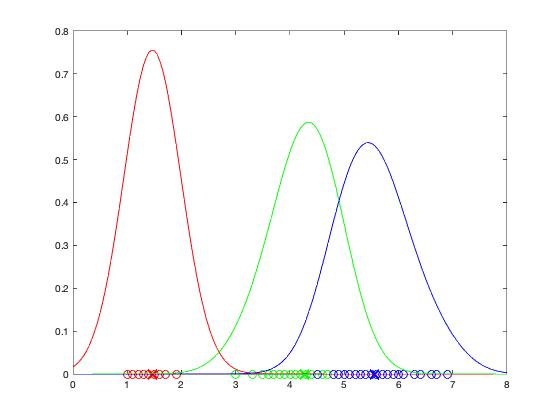
\includegraphics[width=7.6cm]  {gaussianIris0_5.jpg}  \label{fig:gaussianIris0_5}}
    		%\hspace{0.1pc}
    		\caption{Iris Data - Petal Length with Setosa in Red, Versicolor in Green and Virginica in Blue}
    		\label{fig:1D_Parzen}
	\end{center}
\end{figure}

\begin{figure}[htbp]
	\begin{center}
    		\subfigure[Gaussian Kernel with h = 0.1] {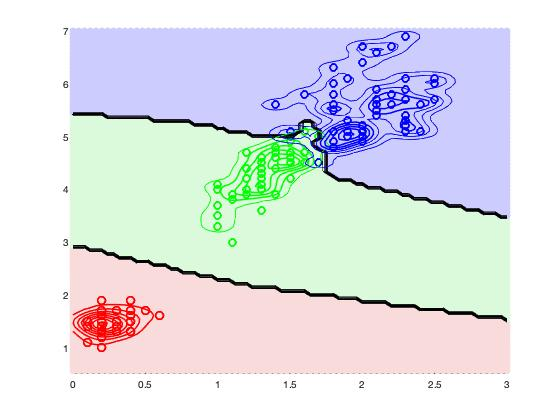
\includegraphics[width=7.6cm]  {gaussianIris2_0_1.jpg}  \label{fig:gaussianIris0_1}}\\
    		%\hspace{0.1pc}
		\subfigure[Gaussian Kernel with h = 0.25] {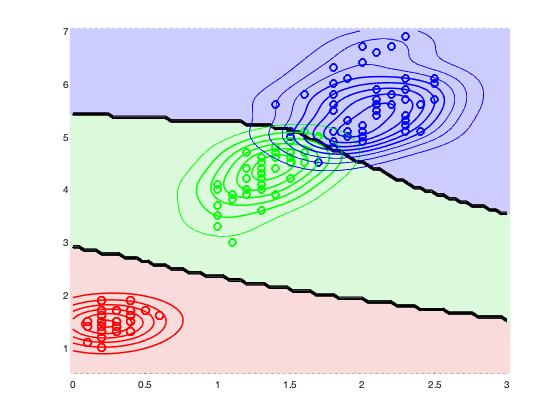
\includegraphics[width=7.6cm]  {gaussianIris2_0_25.jpg}  \label{fig:gaussianIris0_25}}
    		%\hspace{0.1pc}
		\subfigure[Gaussian Kernel with h = 0.5] {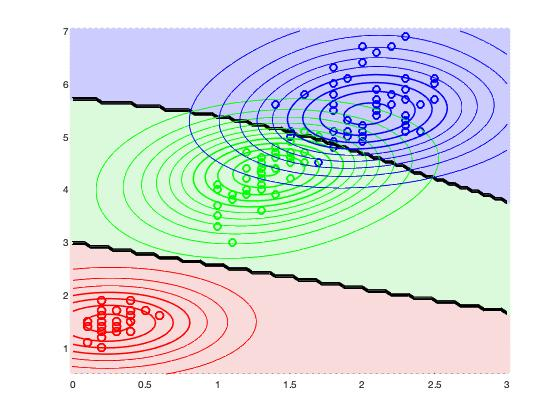
\includegraphics[width=7.6cm]  {gaussianIris2_0_5.jpg}  \label{fig:gaussianIris0_5}}
    		%\hspace{0.1pc}
    		\caption{Iris Data - Petal Length vs Petal Width with Setosa in Red, Versicolor in Green and Virginica in Blue}
    		\label{fig:2D_Parzen}
	\end{center}
\end{figure}

    
    \vspace{5mm}
    
    \pagebreak
    
       %%%%%%%%%%%%%%%%%%%%%%%%% Problem 5 %%%%%%%%%%%%%%%%%%%%%%%%%%%%%%%%%%%%%%%

\textbf{References}

\begin{enumerate} 
	\item[{[1]}] Bishop, Christopher M., \textit{Neural Networks for pattern Recognition}, Oxford University Press, 1995 
	\item[{[2]}] Bishop, Christopher M., \textit{Pattern Recognition and Machine Learning}, Springer, 2006, \\
	https://www.microsoft.com/en-us/research/uploads/prod/2006/01/Bishop-Pattern-Recognition-and-Machine-Learning-2006.pdf
	\item[{[3]}] Duin, Robert P.W., Tax, David and Pekalska, Elzbieta, \textit{PRTools}, http://prtools.tudelft.nl/
	\item[{[4]}] Dempster, A. P., Laird, N. M. and Rubin, D. B., \textit{Maximum likelihood from incomplete data via the EM algorithm}, Journal of the Royal Statistical Society B, Volume 39, Number 1, pp.1–22, 1977
	\item[{[5]}] Franc, Vojtech and Hlavac, Vaclav, \textit{Statistical Pattern Recognition Toolbox}, \newline https://cmp.felk.cvut.cz/cmp/software/stprtool/index.html
	\item[{[6]}] Fukunaga, Keinosuke, \textit{Introduction to Statistical Pattern Recognition}, Academic Press, 1972 
	\item[{[7]}] Goodfellow, Ian, Bengio, Yoshua, and Courville, Aaron, \textit{Deep Learning}, MIT Press, 2016
	\item[{[8]}] Russell, S., and Norvig, P., \textit{Artificial Intelligence A Modern Approach}, $4^{th}$ Edition, Pearson, 2020
	\item[{[9]}] Tomasi, C., \textit{Estimating Gaussian Mixture Densities with EM – A Tutorial}, Duke University Course Notes, 2006, http://www.cs.duke.edu/courses/spring04/cps196.1/handouts/EM/tomasiEM.pdf, Retrieved Sept 2006
\end{enumerate}



\end{enumerate}
\end{document}
